%
\chapter{Fundamentals}\label{cha:Fundamentals}
%
%Eine wissenschaftliche Abschlussarbeit kann im Allgemeinen in die folgenden 4 Phasen gegliedert werden.
%
\section{Properties of Truck at Carola-Cup}\label{sec:Properties of Truck at Carolo-Cup}
%
The Carolo-Cup is an annual competition at the Technical University of Braunschweig which are attended by students. Every year the truck and some properties of the competition are changing. For example, in the competitions until 2017 there was no traffic sign, but starting in 2017 there are also some traffic signs, speed limit zones, blocked areas and crosswalks for pedestrian. Because of this, in the competitions until 2017, there was only one way to understand who had the right of way. If there is a stop line on the road in front of an intersection, it means the car has to wait until the intersection is free. In the competitions starting from 2017, the intersections are in different parts: They are 'Intersections with stop lines', 'Intersections with give-way lines', 'Intersections with priority to right', 'Enforced crossing direction - give-way condition', 'Enforced crossing direction - right of way condition'. Except 'Intersections with priority to right', they all have traffic signs stating who has priority. If there is a no traffic sign, it means the right side always has priority.

\begin{figure}[H]
	\centering
	\hspace*{0cm}   
	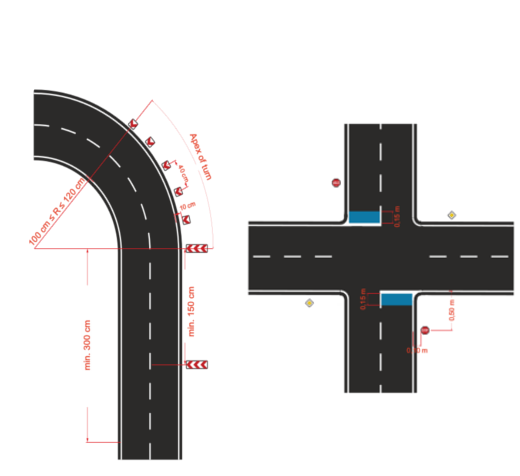
\includegraphics[width=120mm,scale=1]{./Bilder/Intersections.png}
	\caption{Left: Markings for sharp turns at Carolo-Cup.
Right: Intersections with stop lines at Carolo-Cup}
\end{figure}

%
\section{Inverse Perspective Mapping}\label{sec:Inverse Perspective Mapping}
%
Inverse Perspective Mapping(IPM) is an algorithm which is able to obtain accurate bird's-eye view images from the sequential of forward looking cameras. With the IPM algorithm, each image pixel is remapped, and a new array of pixels is created where the lines in perspective are transformed into straight lines and objects are distorted. IPM is one of the most used methods in lane detection. In lane detection, IPM ensures that the lanes are shown vertical and parallel to each other. On the other hand, because of the re-mapping of pixels, IPM is a computationally expensive method. Because of this reason, in some cases in this master's thesis, rather than remapping all pixels of the images, only the pixels relevant to the lane and accordingly, the fitted curve, were remapped. Thanks to this, in some cases, a lot of computing time was saved.

In order to use the IPM method, the intrinsic and extrinsic parameters of camera are necessary to process images for coordinate transformation and calibration.

\begin{itemize}

\item \textbf{Intrinsic Parameters :} Intrinsic parameters are camera-specific. It includes
information of the focal length ($f_x$, $f_y$) and optical centers ($c_x$, $c_y$). It is also called a camera matrix. Although the intrinsic parameters are camera-specific, once the camera is calibrated, the modified intrinsic parameters can be stored for future purposes. It is expressed as a 3x3 matrix:

 \begin{center}
  camera matrix =  $
 \begin{bmatrix} 
f_x & 0 & c_x \\
0 & f_y & c_y \\
0 & 0 & 1 \\
\end{bmatrix}
$  \end{center}

\item \textbf{Extrinsic Parameters :} Extrinsic parameters are dependent on the camera position. The parameters are H and $\theta$. H is the distance between the camera and ground. $\theta$ is the camera tilt angle. 
 
\end{itemize}
  
  
\begin{figure}[H]
\centering
  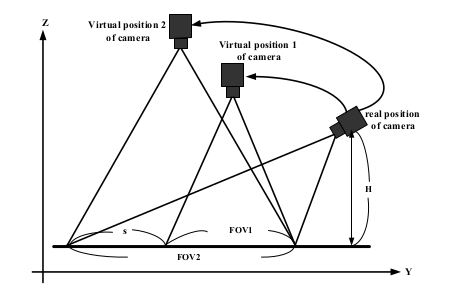
\includegraphics[width=0.8\textwidth]{./Bilder/Related_positions_of_the_camera.png}\label{Procedures_of_IPM}
  \caption{Related Positions of the Camera \cite{IPM}}
\end{figure}

 As seen at \ref{Procedures_of_IPM}, the camera on the car has field of view 2(FOV2) at the real position of the camera but in this case, the view is not a bird's-eye view, so if the same FOV is to be observed from a bird's-eye view, IPM will virtually change the position to Virtual Position 2 of the camera. In this case, although the camera is at its real position, it will appear as though it is at Virtual Position 2. For that, the image coordinates must also be changed. Below, the steps of IPM calculations from the paper of \cite{IPM} will be detailed.
 
In the formula, the original image coordinates will be defined as (x,y), the destination image coordinates will be defined as ($x^*$,$y^*$), the distance between the ground and the camera will be defined as H, the focal length of camera will be defined as f, and the tilt angle of camera will be defined as $\theta$.
 
\begin{center}
 $x^* = H \frac{x sin \theta + f cos \theta}{-y cos \theta + f sin \theta}$ ;
 $y^* = H \frac{y sin \theta + f cos \theta}{-y cos \theta + f sin \theta}$ 
\end{center}

In this equation, the transformed component values of $x^*$ and $y^*$ may be less than or equal to zero. Because of 
this reason, a constant d is defined as $
\begin{vmatrix}
H(sin \theta + cos \theta)/(f sin \theta - cos \theta) 
\end{vmatrix}
$  + 1. This means that the coordinate point in the original source image has been mapped into the point of the destination image coordinate system. Below there is the proposed equation :
 
 \begin{center}
 $x^* = H \frac{x sin \theta + f cos \theta}{-y cos \theta + f sin \theta}$ + d ,
 $y^* = H \frac{y sin \theta + f cos \theta}{-y cos \theta + f sin \theta}$ + d ,
 where d = 
 $\begin{vmatrix}
 \frac{H(sin \theta + f cos \theta)}{f sin \theta - cos \theta}
 \end{vmatrix}$ + 1
\end{center}

\begin{figure}[H]
 \centering
  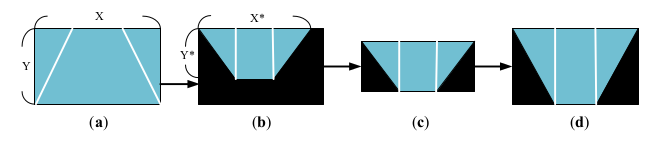
\includegraphics[width=1\textwidth]{./Bilder/Procedures_of_IPM.png}\label{Procedures_of_IPM}
  \caption{Procedures of IPM}
\end{figure}


%
\section{Edge Detection}\label{sec:Edge Detection}
%

Edge detectors are essential parts of most computer vision systems. Edge detectors dramatically decrease the amount of data to be processed and extract the useful parts of images. They work by detecting discontinuities in brightness. In this project, the edge detector was used in order to detect the lanes and to exclude unnecessary information from images. There are different methods for edge detection, but they can be grouped into two categories. They are :

\begin{itemize}

\item \textbf{Gradient method : } This method searches for the maximum and minimum in the first derivative of the image and with that, the edges can be found. For this method, the first order derivative filter must be used. For example : Sobel-Operator.
 
\item \textbf{Laplacian method : } This method searches for the zero crossing in the second derivative of the image and with that, the edges can be found. For this method, the second order derivative filter must be used. For example : Laplacian Filter. 
  
\end{itemize}
 
According to \cite{Machine_Vision},here are three steps of the edge detection algorithm. They are :

\begin{itemize}

\item \textbf{Filtering : } For edge detection, it is required to use a suitable smoothing filter. The filters sharpen the edges and ignore the unnecessary information. It is often utilized to improve the functioning of an edge detector against noise. The more filtering is applied, however, the greater the loss of edge strength.
 
\item \textbf{Enhancement : } To be able to better detect edges, changes in the intensity in the area surrounding a point must be determined. Pixels in which a significant change in intensity occurs are emphasized by enhancement, which is usually applied by calculating the gradient magnitude.
  
\item \textbf{Detection : } Though many points in an image have a nonzero value for the gradient, not all of these points are actually edges. Because only points with strong edge content are desired, a method must be applied to determine which points are actual edge points. Thresholding is often utilized to do so.
 
\end{itemize}

Well known smoothing filters are :

\begin{itemize}

 \item Sobel-Operator
 \item Canny Edge Detector
 \item Laplacian-Filter
 \item Prewitt-Operator
 
 \end{itemize}
 
In this master's thesis, the Sobel Operator was utilized, so it will be described in more detail.

%
\subsection{Sobel Operator}\label{sec:Sobel Operator}

The Sobel Operator, sometimes called the Sobel filter is one of the most used edge detectors in image processing and computer vision. The Sobel Operator uses vertical and horizontal masks. These masks used are odd-numbered square matrices and they are generally 3x3 matrices. \emph{\color{red}The operator uses two 3x3 kernels which are convolved with the original image to calculate approximations of the derivatives - one for horizontal changes, and one for vertical. If we define A as the source image, and $G_{x}$ and $G_{y}$ are two images which at each point contain the horizontal and vertical derivative approximations respectively, the computations are as follows:}

\[
  G_{x} = 
  \begin{bmatrix}
	+1 & 0 & -1 \\
	+2 & 0 & -2 \\
	+1 & 0 & -1 \\
   \end{bmatrix} * A  \quad
  G_{y} = 
  \begin{bmatrix}
	+1 & +2 & +1 \\
	0 & 0 & 0 \\
	+1 & -2 & -1 \\
  \end{bmatrix} * A
\]

where * here denotes the 2-dimensional signal processing convolution operation.

Since the Sobel kernels can be decomposed as the products of an averaging and a differentiation kernel, they compute the gradient with smoothing. For example, \textbf{$G_{x}$}  can be written as

$  \begin{bmatrix}
	+1 & 0 & -1 \\
	+2 & 0 & -2 \\
	+1 & 0 & -1 \\
   \end{bmatrix} =  \begin{bmatrix}
	1 \\
	2 \\
	1 \\
  \end{bmatrix} \begin{bmatrix}
	+1 & 0 & -1
  \end{bmatrix}
$

The x-coordinate is defined here as increasing in the 'right'-direction, and the y-coordinate is defined as increasing in the 'down'-direction. At each point in the image, the resulting gradient approximations can be combined to give the gradient magnitude, using:

G = $\sqrt{ G_{x}^{2} + G_{y}^{2} }$

Using this information, we can also calculate the gradient's direction:

$\theta = atan(\dfrac{G_{y}}{G_{x}})$

where, for example, $\theta$ is 0 for a vertical edge which is lighter on the right side.\cite{Sobel_Operator}






\begin{figure}[H]
  \centering
  \subfloat[Original Image]{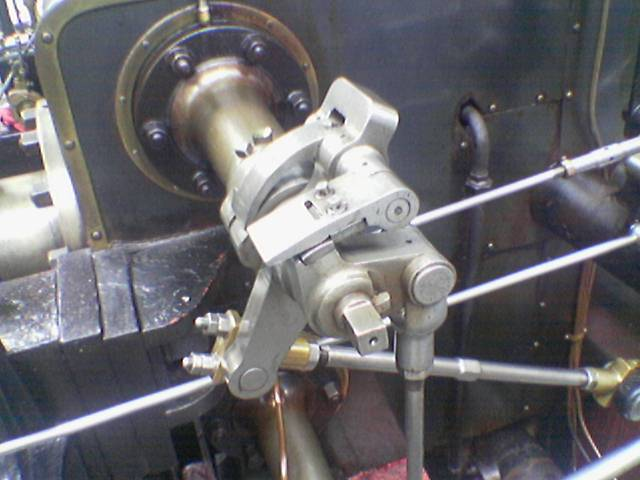
\includegraphics[width=0.4\textwidth]{./Bilder/Sobel_Original.png}\label{fig:f1}}
  \hfill
  \subfloat[Sobel Operator applied Image]{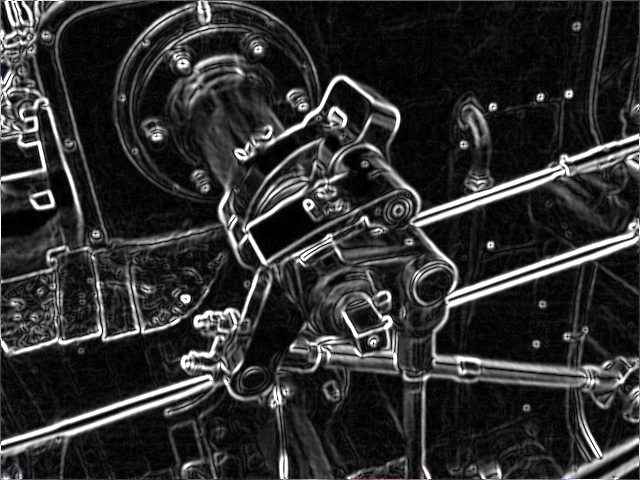
\includegraphics[width=0.4\textwidth]{./Bilder/Sobel_Operator.png}\label{fig:f2}}
  \caption{Sobel Operator\cite{Sobel_Operator}}
\end{figure} 


%
\subsection{Canny Edge Detector}\label{sec:Canny Edge Detector}

Canny edge detector was developed in 1986 and called with the name of its developer John F. Canny. Canny edge detector is also so popular edge detector like Sobel operator. Canny edge detector is a multi-stage algorithm and it can be analyzed in 5 different stages.\cite{Canny_Edge_Detector2}

\begin{enumerate}
\item \textbf{Noise Reduction : } To get so stabile lane detection results, we have to reduce/remove all noise from frames. Lane detection without filter out the noise can cause false detection. Gaussian filter is used for removing noise in the frames. Gaussian filter blurs images and remove detail and noise. The size of Gaussian filter kernel must be (2k+1)x(2k+1). It is important to choose the size of Gaussien filter because if the size of kernel is larger, detector's sensitivity to noise is lower but on the other hand,\emph{\color{red} the localization error to detect the edge will slightly increase with the increase of the Gaussian filter kernel size.} \cite{Canny_Edge_Detector}

\item \textbf{Finding Intensity Gradient of the Image : } \emph{\color{red}The Canny algorithm basically finds edges where the grayscale intensity of the image changes the most. These areas are found by determining gradients of the image. Gradients at each pixel in the smoothed image are determined by applying what is known as the Sobel operator. Sobel operator has already explained in section \ref{sec:Sobel Operator}.}


\item \textbf{Non-maximum Suppression : }
\item \textbf{Double Thresholding : }
\item \textbf{Hysteresis Thresholding : }
\end{enumerate}


\begin{figure}[H]
  \centering
  \subfloat[Original Image]{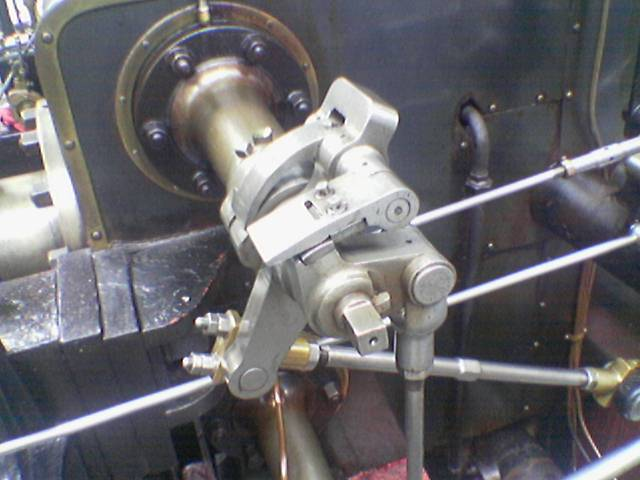
\includegraphics[width=0.4\textwidth]{./Bilder/Sobel_Original.png}\label{fig:f1}}
  \hfill
  \subfloat[Canny Edge Detector applied Image]{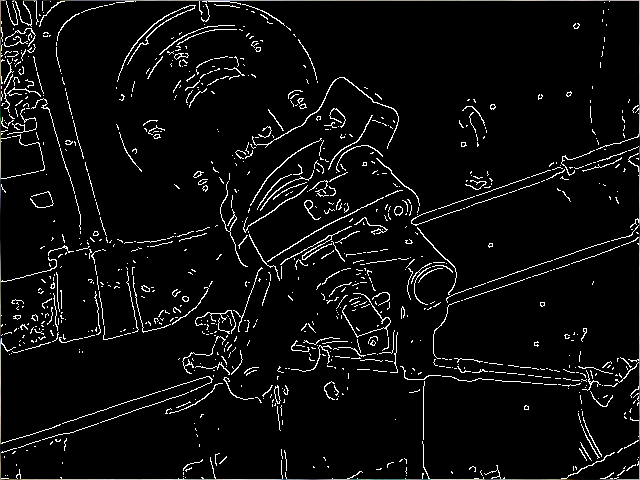
\includegraphics[width=0.4\textwidth]{./Bilder/Canny_Edge_Detector.png}\label{fig:f2}}
  \caption{Canny Edge Detector\cite{Canny_Edge_Detector}}
\end{figure} 





%
\section{Hough-Transformation}\label{sec:Hough-Transformation}
%

%
\subsection{Standart Hough-Transformation}\label{sec:Standart Hough - Transformation}
%


%
\subsection{Probabilistic Hough-Transformation}\label{sec:Probabilistic Hough-Transformation}
%




%
\section{K-Nearest Neighbors Algorithm}\label{sec:K-Nearest Neighbors Algorithm}
%
K-Nearest Neighbor(KNN) is an non-parametric lazy learning algorithm. The non-parametric technique means that it doesn't make any assumptions on the underlaying data distribution. In the definition of KNN, the term 'lazy learning algorithm' is used. It means it doesn't use the data training points to do any generalization. In other words, there is no explicit training phase or it is very minimal.  It also means that the training phase is pretty fast. Most of the lazy algorithms - especially KNN - make decisions based on the entire training data set. On the other hand, KNN is one of the top 10 data mining algorithms\cite{k_nearest_neighbors}.

\begin{figure}[H]
 \centering
  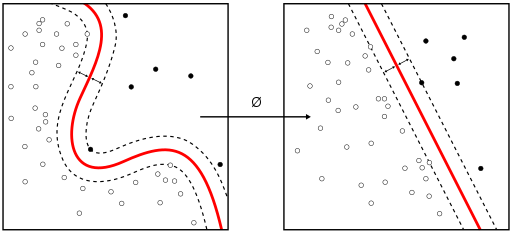
\includegraphics[width=1\textwidth]{./Bilder/k-nearest-neighbors.png}\label{Procedures_of_IPM}
  \caption{K-Nearest-Neighbors Algorithm\cite{k_nearest_neighbors_wikipedia}}
\end{figure}

The K-Nearest Neighbors Algorithm has advantages and disadvantages. According to \cite{k_nearest_neighbors_adv_disadv},the main advantages of KNN are simplicity, effectiveness, intuitiveness and competitive classification performance in many domains. On the other hand, KNN can have poor run-time performance when the training set is large. It is very sensitive to irrelevant or redundant features because all features contribute to the similarity and thus to the classification. The computation cost is also quite high because we need to compute distance of each query instance to all training samples. 

%
\section{Curve Fitting}\label{sec:Curve Fitting}

\emph{\color{red}Curve fitting is used to find the 'best fit' line or curve for a series of data points. Curve fitting produces mostly mathematical equations that can be used to find points anywhere along
the curve.\cite{Curve_Fitting}} They are several different types of curve fitting. Some of them are: linear, exponential, polynomial, exponential, power, logarithmic, etc. In this master thesis, polynomial curve fitting was used. Polynomial curve fitting differs from order of the polynomial. Polynomial curve fittings are called different names depending on their orders. First order polynomial curve fittings are called linear regression, second order as quadratic regression, and third order as cubic regression.

\begin{figure}[H]
 \centering
  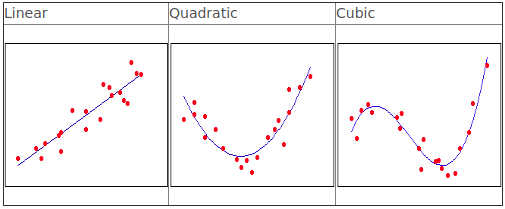
\includegraphics[width=1\textwidth]{./Bilder/Curve_Fitting_Polynomial.png}\label{Curve_Fitting_Polynomial}
  \caption{Types of Polynomial Curve Fitting\cite{Curve_Fitting_Polynomial}}
\end{figure}

%




